
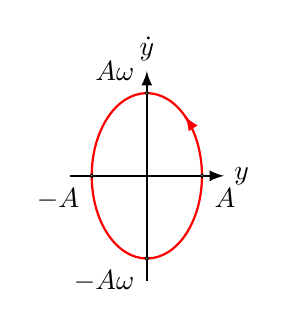
\begin{tikzpicture}[>=latex, scale=0.7]

  % Ellipse
  \draw[thick, red] (0,0) ellipse (1 and 1.5);

  % Achsen
  \draw[->, thick] (-1.4,0) -- (1.4,0) node[right] {$y$};
  \draw[->, thick] (0,-1.9) -- (0,1.9) node[above] {$\dot{y}$};

  % Beschriftungen
  \node at (1,0) [below right=1pt] {$A$};
  \node at (-1,0) [below left=1pt] {$-A$};
  \node at (0,1.5) [above left=1pt] {$A\omega$};
  \node at (0,-1.5) [below left=1pt] {$-A\omega$};

  % Punkte auf Ellipse
  \filldraw[white, draw=black] (1,0) circle (0.03);
  \filldraw[white, draw=black] (-1,0) circle (0.03);
  \filldraw[white, draw=black] (0,1.5) circle (0.03);
  \filldraw[white, draw=black] (0,-1.5) circle (0.03);

  % Pfeil auf der Ellipse
  \draw[->, red, thick, domain=45:46] plot ({cos(\x)}, {1.5*sin(\x)});
\end{tikzpicture}